\item \textbf{{[}ACJC/PRELIM/9569/2021/P1/Q6{]} }

A driving simulator is programmed using Object-Oriented Programming
(OOP).

The diagram below shows a UML Class Diagram with \textbf{some} of
the classes, attributes, and methods used in the simulator.
\noindent \begin{center}
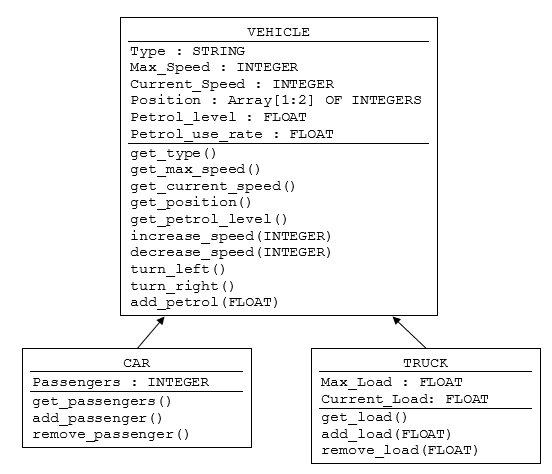
\includegraphics[scale=0.8]{C:/Users/Admin/Desktop/Github/question_bank/LyX/static/img/9569-ACJC-2021-P1-Q6}\quad{}
\par\end{center}
\begin{enumerate}
\item State the relationship between the \texttt{CAR} class and the \texttt{VEHICLE}
class. \hfill{}{[}1{]}
\item Explain briefly, in this context, how each of the following features
of Object-Oriented Programming help the simulation to be developed
more efficiently.
\begin{enumerate}
\item Abstraction \hfill{} {[}2{]}
\item Inheritance \hfill{}{[}2{]}
\end{enumerate}
\item The petrol use rate depends on the speed at which the vehicle is travelling,
as well as the mass of the vehicle and the contents of the vehicle
-- the number of passengers in a car, or the mass of the load in
a truck. Explain how polymorphism can be used in this case to write
the simulation. \hfill{}{[}2{]}
\end{enumerate}